%\title{LaTeX Portrait Poster Template}
%%%%%%%%%%%%%%%%%%%%%%%%%%%%%%%%%%%%%%%%%
% a0poster Portrait Poster
% LaTeX Template
% Version 1.0 (22/06/13)
%
% The a0poster class was created by:
% Gerlinde Kettl and Matthias Weiser (tex@kettl.de)
% 
% This template has been downloaded from:
% http://www.LaTeXTemplates.com
%
% License:
% CC BY-NC-SA 3.0 (http://creativecommons.org/licenses/by-nc-sa/3.0/)
%
%%%%%%%%%%%%%%%%%%%%%%%%%%%%%%%%%%%%%%%%%

%----------------------------------------------------------------------------------------
%	PACKAGES AND OTHER DOCUMENT CONFIGURATIONS
%----------------------------------------------------------------------------------------

\documentclass[a0,portrait]{a0poster}

\usepackage{multicol} % This is so we can have multiple columns of text side-by-side
\columnsep=100pt % This is the amount of white space between the columns in the poster
\columnseprule=3pt % This is the thickness of the black line between the columns in the poster

\usepackage[svgnames]{xcolor} % Specify colors by their 'svgnames', for a full list of all colors available see here: http://www.latextemplates.com/svgnames-colors

\usepackage{times} % Use the times font
%\usepackage{palatino} % Uncomment to use the Palatino font

\usepackage{graphicx} % Required for including images
\graphicspath{{figures/}} % Location of the graphics files
\usepackage{booktabs} % Top and bottom rules for table
\usepackage[font=small,labelfont=bf]{caption} % Required for specifying captions to tables and figures
\usepackage{amsfonts, amsmath, amsthm, amssymb} % For math fonts, symbols and environments
\usepackage{wrapfig} % Allows wrapping text around tables and figures

\usepackage{listings}
\usepackage{xcolor}
\usepackage{amssymb}
 \usepackage{amsthm}
 \usepackage{amsfonts}
\usepackage{braket}
\DeclareCaptionFont{white}{\color{white}}
\DeclareCaptionFormat{listing}{%
\parbox{\textwidth}{\colorbox{gray}{\parbox{\textwidth}{#1#2#3}}\vskip-4pt}}
\captionsetup[lstlisting]{format=listing,labelfont=white,textfont=white}
\lstset{frame=lrb,xleftmargin=\fboxsep,xrightmargin=-\fboxsep, columns=fullflexible}
\begin{document}

%----------------------------------------------------------------------------------------
%	POSTER HEADER 
%----------------------------------------------------------------------------------------

% The header is divided into two boxes:
% The first is 75% wide and houses the title, subtitle, names, university/organization and contact information
% The second is 25% wide and houses a logo for your university/organization or a photo of you
% The widths of these boxes can be easily edited to accommodate your content as you see fit

\begin{minipage}[b]{0.8\linewidth}
\VeryHuge \color{NavyBlue} \textbf{Analysis of \textit{Chaos Game} simulations with Pygame} \color{Black}\\ % Title
\Huge\textit{}\\[2.4cm] % Subtitle
\huge \textbf{Indranil Ghosh}\\[0.7cm] % Author(s)
\huge \textit{Jadavpur University, Department of Physics}\\[0.4cm] % University/organization
\Large \texttt{indranilg49@gmail.com} --- +91 7550 860 174\\
\end{minipage}
%
\begin{minipage}[b]{0.4\linewidth}
\includegraphics[height=12cm]{logo.jpg}\\
\end{minipage}

\vspace{0.5cm} % A bit of extra whitespace between the header and poster content

%----------------------------------------------------------------------------------------

\begin{multicols}{3} % This is how many columns your poster will be broken into, a portrait poster is generally split into 2 columns

%----------------------------------------------------------------------------------------
%	ABSTRACT
%----------------------------------------------------------------------------------------

\color{Red} % Navy color for the abstract

\begin{abstract}
This project is based on the dynamic simulations of various Chaos Game algorithms to produce fractal patterns, with the help of Pygame. Patterns to be discussed are Sierpinski’s Triangle, Barnsley’s fern and few restricted chaos game fractals. The Chaos game makes use of a random process to produce visualizations of self-similar fractal patterns on a plane. In this project some of the few fractal patterns, each with a description , its own chaos game rule and Pygame codes, to simulate its development are listed. Now, Pygame is a cross-platform set of python modules to create interactive video-games. These Pygame simulators make the visualizations of the pattern-generation grow with time, and very beautiful to look at. I also discuss some of the norms to be followed while using Pygame and its applications in scientific programming. 
\end{abstract}
%----------------------------------------------------------------------------------------
%	INTRODUCTION
%----------------------------------------------------------------------------------------

\color{Black} % SaddleBrown color for the introduction
\section*{Introduction}
The algorithm of \textit{Chaos Game} was first developed by the british mathematician, \textbf{Michael Barnsley} around the year 1988, which produced some interesting fractal patterns. Generally, it refers to the method of generating the fixed point (attractor) of an iterated function system(IFS). Using the algorithm, the pattern is produced by iteratively creating a sequence of points, starting with an initial random point anywhere on the drawing platform. In the sequence, each point is the fraction of the distance between the previous point and a randomly chosen vertex (by rolling a dice, if human or by using a pseudo-random generator, if a computer!) of the n-gon.\\
\begin{itemize}
\item Although the algorithm is quite simple, the patterns formed, after continuous iterations, always exhibit infinite complexity and self similarity. Zooming a particular section of the fractal, results in the same pattern but with less density of points.\\
\item When the simulations are carried out, the fractal patterns grow and become clearer with time, with each iterations. If the n-gon is regular, the pattern formed is symmetric.
\end{itemize}
%----------------------------------------------------------------------------------------
%	GEOLOGY
%----------------------------------------------------------------------------------------

\color{Black} % DarkSlateGray color for the rest of the content

\section*{Sierpinski's Triangle}
Coined by the Polish mathematician \textbf{Waclaw Sierpinski}, this triangle needs 3 random vertces and a random starting point to start with the simulation. The distance factor \textbf{r} is $\frac{1}{2}$. Let A, B and C be the 3 random vertices of a triangle and St be the starting point,  also chosen randomly on the drawing platform. Playing with rolling a dice, we come up with any random integer in the range [1, 6] with an equal probability $\frac{1}{6}$. We design the game in such a way that, if we come up with a face \textbf{1 or 2}, we move towards point \textbf{A} from the previous point and plot a new point halfway between. SImilarly for faces \textbf{3 or 4} or \textbf{5 or 6}, we move halfway towards \textbf{B} or \textbf{C} respectively. The process continued for a large number of iterations results in Figure 1.
\begin{center}\vspace{0.5cm}
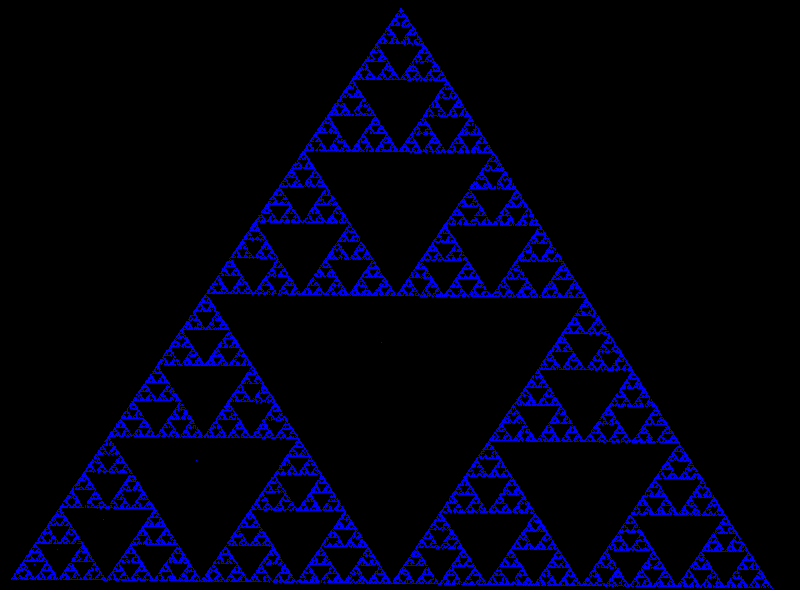
\includegraphics[width=0.6\linewidth]{sier}
\captionof{figure}{\color{Blue} Simulation of Sierpinski's Triangle}
\end{center}%\vspace{1cm}
%----------------------------------------------------------------------------------------
%	GEOTHERMAL DATA
%----------------------------------------------------------------------------------------
\subsection*{Code snippet}
\begin{lstlisting}[language=Python, frame=single]
import random, pygame, sys
from pygame.locals import*
#set up the window
DISPLAYSURF=pygame.display.set_mode((800, 800))
#set up the colors
BLACK=(0, 0, 0)
BLUE=(0, 0, 255)
i=0
while True:
    for event in pygame.event.get():
        if event.type==QUIT:
            pygame.image.save(DISPLAYSURF, "Sierpinski.png")
            pygame.quit()
            sys.exit()
        elif event.type==MOUSEBUTTONUP:
            i+=1
            if i==1:
                A=(event.pos[0], event.pos[1])
                pygame.draw.circle(DISPLAYSURF,BLUE,A,0,0)
            elif i==2:
                B=(event.pos[0], event.pos[1])
                pygame.draw.circle(DISPLAYSURF,BLUE,B,0,0)
            elif i==3:
                C=(event.pos[0], event.pos[1])
                pygame.draw.circle(DISPLAYSURF,BLUE,C,0,0)
            elif i==4:
                St=(event.pos[0], event.pos[1])
                pygame.draw.circle(DISPLAYSURF,BLUE,St,0,0)
            else:
                pygame.quit()
                sys.exit()
    if i==4:
        x=random.randint(1, 6)
        if x in [1, 2]: St=((St[0]+A[0])//2, (St[1]+A[1])//2)
        elif x in [3, 4]: St=((St[0]+B[0])//2, (St[1]+B[1])//2)
        else: St=((St[0]+C[0])//2, (St[1]+C[1])//2)
        pygame.draw.circle(DISPLAYSURF, BLUE, St, 0, 0)
    pygame.display.update()
\end{lstlisting}

\begin{itemize}
\item The Hausdorff Dimension of Sierpinski's Triangle is 1.5849.
\end{itemize}
%\subsection*{Heat Flow}
%\begin{itemize}
%\item Average heat flow values are 82$\pm19$ mW/m$^2$
%\item Very high heat flow values (90-130 mW/m$^2$) in South Algeria (Hoggar Precambrian basement).
%\end{itemize}
%\begin{center}\vspace{1cm}
%\includegraphics[width=1.0\linewidth]{qpd4}
%\captionof{figure}{\color{Green} (A) Temp. vs. depth for different regions (Takherist and Lesquer, 1989). (B) Heat flow map of Algeria (Takherist and Lesquer, 1989). Unit: mW/m$^2$. 230 oil wells are presented, with depths ranging from 500 to 5500 m.}
%\end{center}\vspace{1cm}

%------------------------------------------------

\section*{number of vertices=5, r=$\frac{1}{2}$}
%\begin{enumerate}
%\item The Tlemcenian dolomites in the NW-Algeria: thermal waters are related to the Plio-Quaternary volcanic rocks; bicarbonate water type.
%\item Carbonate formations in the NE-Algeria: area is 15,000 km$^2$; high flow rates (\textgreater100 L/s); highest temperature in Algeria (98 $^{\circ}$C). 
%\item Albian sandstone reservoir in the South of Algeria: area is 600,000 km$^2$; depth of aquifer is 2.6 km; highly mineralized waters.
%\end{enumerate}
\begin{center}\vspace{0.4cm}
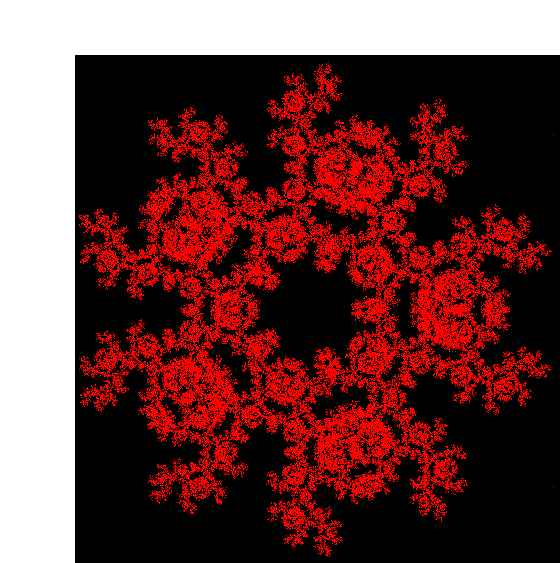
\includegraphics[width=0.5\linewidth]{Penta}
\captionof{figure}{\color{Blue}A restricted Pentagon}
\end{center}\vspace{1cm}

\subsection*{number of vertices=6, r=$\frac{1}{3}$}
\begin{center}\vspace{0.4cm}
\includegraphics[width=0.5\linewidth]{Hexa}
\captionof{figure}{\color{Blue}A Hexagon}
\end{center}\vspace{1cm}
\begin{itemize}
\item The Hausdorff Dimension of this pattern is 1.6309.
\end{itemize}
\section*{Barnsley's fern}
\begin{itemize}
\item Devised by Michael Barnsley, the computer code that simulates this pattern is also an example of IFS (iterated Function System).
\item The algorithm developed by Barnsley also follows from the \textit{collage theorem}.
\item To construct the leaf, we need these four affine transformations:\\
\begin{gather}
f_1(x, y)=\begin{bmatrix}0.00 & 0.00 \\ 0.00 & 0.16 \end{bmatrix}\begin{bmatrix}x\\y\end{bmatrix}
\end{gather}
\begin{gather}
f_2(x, y)=\begin{bmatrix}0.85 & 0.04 \\ -0.04 & 0.85 \end{bmatrix}\begin{bmatrix}x\\y\end{bmatrix} + \begin{bmatrix}0.00\\1.60\end{bmatrix}
\end{gather}
\begin{gather}
f_3(x, y)=\begin{bmatrix}0.20 & -0.26 \\ 0.23 & 0.22 \end{bmatrix}\begin{bmatrix}x\\y\end{bmatrix} + \begin{bmatrix}0.00\\1.60\end{bmatrix}
\end{gather}
\begin{gather}
f_4(x, y)=\begin{bmatrix}-0.15 & 0.28 \\ 0.26 & 0.24 \end{bmatrix}\begin{bmatrix}x\\y\end{bmatrix} + \begin{bmatrix}0.00\\0.44\end{bmatrix}
\end{gather}
\item In simulating the growth, the first point is drawn at the origin ($X_0=0$, $Y_0=0$) and the successive points are iteratively plotted by randomly choosing one of the above four transformations.
\item $f_1$ transformation is chosen $1\%$ of the times and maps the base of the stem of the leaf, $f_2$ is chosen $85\%$ of the times and maps the smaller leaflets, $f_3$ and $f_4$ are each chosen $7\%$ of the times and maps the largest left-handed and the largest right-handed leaflet respectively.
\end{itemize}

\begin{center}\vspace{0.5cm}
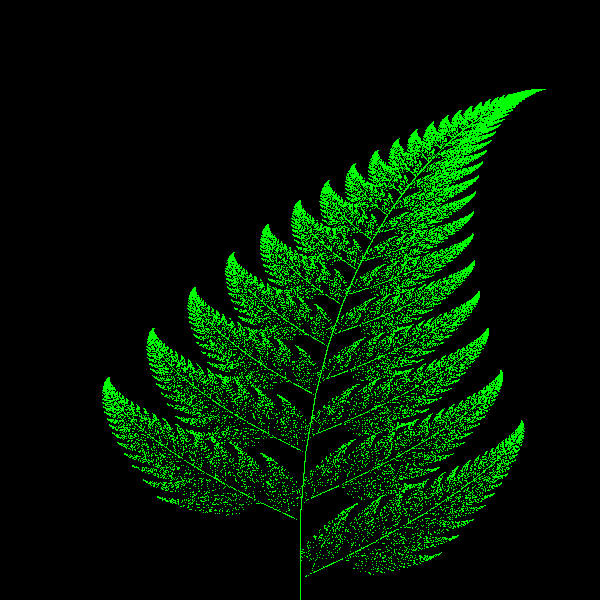
\includegraphics[width=0.6\linewidth]{BarnsleyFern}
\captionof{figure}{\color{Blue}Barnsley's Fern, type: \textbf{\textit{Black Spleenwort}}}
\end{center}\vspace{0.5cm}

\subsection*{Code Snippet}
\begin{lstlisting}[language=Python, frame=single]
GREEN=(0, 255, 0)

X=[0.0]
Y=[0.0]
i=0

while True:
    r=random.random() 
    if r<=0.02:
        X+=[0.0, ]
        Y+=[0.16*Y[i], ]
    elif r<=0.86:
        X+=[0.85*X[i] + 0.04*Y[i], ]
        Y+=[-0.024*X[i] + 0.85*Y[i] + 1.6, ]
    elif r<=0.93:
        X+=[0.20*X[i] - 0.26*Y[i], ]
        Y+=[0.23*X[i] + 0.22*Y[i] + 1.6, ]
    else:
        X+=[-0.15*X[i] + 0.28*Y[i], ]
        Y+=[0.26*X[i] + 0.24*Y[i] + 0.44, ]

    pygame.draw.circle(DISPLAYSURF, GREEN, 
(int(X[i]*90 + 300), 600 - int(Y[i]*50)), 0, 0) 
    i+=1
\end{lstlisting}

\subsection*{Yet Another Fern}
\begin{center}\vspace{0.5cm}
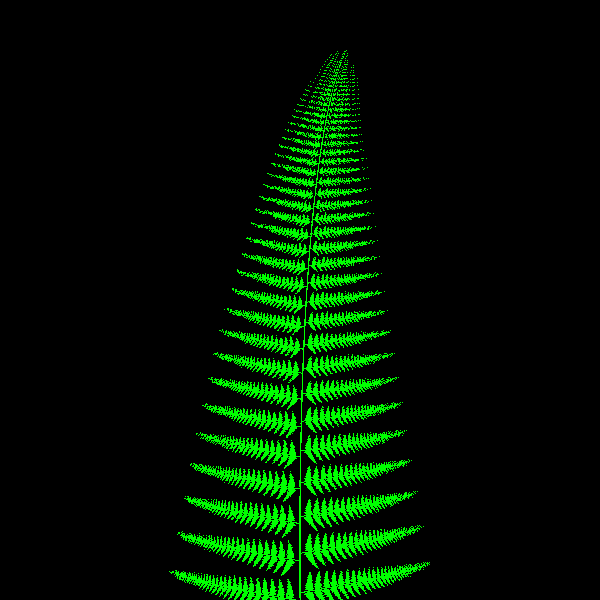
\includegraphics[width=0.5\linewidth]{BarnsleyFern2}
\captionof{figure}{\color{Blue}Barnsley's Fern, type: \textbf{\textit{Thelypteridaceae}}}
\end{center}\vspace{1cm}
%----------------------------------------------------------------------------------------
%	CONCLUSIONS
%----------------------------------------------------------------------------------------

\color{SaddleBrown} % SaddleBrown color for the conclusions to make them stand out

\section*{Conclusions}

\begin{itemize}
\item In our code, we need to keep in mind that the top left corner is coordinated (0, 0) in a pygame drawing surface and the value of Y-axis increases downwards.
\item Pygame does not allow floating point values. So, to get a convinient simulation, we need to map the pygame coordinates to a new coordinate system that suits our needs.
\item The dynamic simulations of fractals have turned out to be useful in scientific applications ranging from computer graphics, image compression, mathematical modeling, in video game industries, etc.
\end{itemize}

\color{Black} % Set the color back to DarkSlateGray for the rest of the content

%----------------------------------------------------------------------------------------
%	FORTHCOMING RESEARCH
%----------------------------------------------------------------------------------------

%\section*{Forthcoming Research}

%Simulation of thermodynamic properties of the thermal fluid and power output with longevity using geological, hydrogeological, and geothermal data from NE-Algerian geothermal reservoirs. 

 %----------------------------------------------------------------------------------------
%	REFERENCES
%----------------------------------------------------------------------------------------

%\nocite{*} % Print all references regardless of whether they were cited in the poster or not
%\bibliographystyle{plain} % Plain referencing style
%\bibliography{sample} % Use the example bibliography file sample.bib

%----------------------------------------------------------------------------------------
\subsection*{Acknowledgement}
I would like to express my special thanks of gratitude to my Professors, Dr. Debasish Lohar and Dr. Subhankar Ray who helped me with useful  suggestions.

\begin{thebibliography}{10}
\bibitem{knuthwebsite}
\texttt{Rubin H. Landau, Manuel Jose Paez and Christian C. Bordeianu, \textit{"Computational Physics"}, New York: Wiley, 2007}
\bibitem{knuthwebsite}
\texttt{Al Sweigart, \textit{"Making Games with Python and Pygame"}, https://github.com/indrag49/Fractals-pygame}
\bibitem{knuthwebsite}
\texttt{Wolfram Mathworld, \textit{"Chaos Game"}, http://mathworld.wolfram.com/ChaosGame.html}
\bibitem{knuthwebsite}
\texttt{Wikipedia, \textit{"Barnsley's Fern"}, https://en.wikipedia.org/wiki/Barnsleyfern}
\bibitem{knuthwebsite}
\texttt{Indranil Ghosh, \textit{"Fractals-pygame"}, https://github.com/indrag49/Fractals-pygame}
\end{thebibliography}

\end{multicols}
\end{document}